\chapter{Đọc thêm 1: SA-MAIS, Bộ Phân tích Cảm xúc Lai cho Thị trường Chứng khoán (Taborda et al.)}
\label{ch:M4L3DT1}

% Nguồn: Taborda, B., et al. ``SA-MAIS: Hybrid automatic sentiment analyser for stock market.'' Journal of Information Science, 2023.
% Phần cần đọc: Toàn bộ bài báo
% Nội dung bắt buộc đọc: được kiểm tra trong mọi bài đánh giá (kể cả Quiz).

\section{Thông tin nguồn}

\begin{itemize}
  \item \textbf{Nguồn:} Taborda, B., Maria de Almeida, A., Carlos Dias, J., Batista, F., \& Ribeiro, R. \emph{SA-MAIS: Hybrid automatic sentiment analyser for stock market}. Journal of Information Science, 2023. \url{https://doi.org/10.1177/01655515231171361}
  \item \textbf{Phần cần đọc:} Toàn bộ nội dung
\end{itemize}

\bigskip
\noindent\textbf{Bruno Taborda}\\
{\small Instituto Universitário de Lisboa (ISCTE-IUL), Bồ Đào Nha; Centre for Informatics and Systems of the University of Coimbra (CISUC), Bồ Đào Nha}

\noindent\textbf{Ana Maria de Almeida}\\
{\small Instituto Universitário de Lisboa (ISCTE-IUL), ISTAR, Bồ Đào Nha; Centre for Informatics and Systems of the University of Coimbra (CISUC), Bồ Đào Nha}

\noindent\textbf{José Carlos Dias}\\
{\small Instituto Universitário de Lisboa (ISCTE-IUL), Bồ Đào Nha; Business Research Unit (BRU-IUL), Bồ Đào Nha}

\noindent\textbf{Fernando Batista}\\
{\small Instituto Universitário de Lisboa (ISCTE-IUL), Bồ Đào Nha; INESC-ID Lisboa, Bồ Đào Nha}

\noindent\textbf{Ricardo Ribeiro}\\
{\small Instituto Universitário de Lisboa (ISCTE-IUL), Bồ Đào Nha; INESC-ID Lisboa, Bồ Đào Nha}

\bigskip
{\small \textbf{Tác giả liên hệ:} Bruno Taborda, ISTAR, Instituto Universitário de Lisboa (ISCTE-IUL), Lisbon 1649-026, Bồ Đào Nha. Email: Bruno\_Taborda@iscte-iul.pt}

\section{Tóm tắt}

Phân tích cảm xúc (sentiment analysis) đối với các tweet liên quan đến thị trường chứng khoán là một nhiệm vụ đầy thách thức, không chỉ vì tính đặc thù của lĩnh vực mà còn vì bản chất ngắn gọn của văn bản. Nghiên cứu này đề xuất SA-MAIS, một phương pháp hai bước nhẹ, được thiết kế riêng để thực hiện phân tích cảm xúc trong các tin nhắn văn bản ngắn bị giới hạn theo lĩnh vực. Để giải quyết vấn đề đặc thù lĩnh vực, dựa trên tần suất xuất hiện của từ, các từ liên quan nhất được tự động trích xuất từ lĩnh vực mới rồi được gắn nhãn thủ công để cập nhật một từ điển cảm xúc (lexicon) đặc thù lĩnh vực đã có sẵn. Sau đó, cảm xúc được phân loại bằng cách kết hợp từ điển đặc thù lĩnh vực đã cập nhật với VADER, một công cụ phân tích cảm xúc nổi tiếng và được sử dụng rộng rãi. Phương pháp đề xuất được so sánh với các công cụ phân tích cảm xúc nổi tiếng và được sử dụng rộng rãi khác, bao gồm các mô hình dựa trên transformer như BERTweet, Twitter-roBERTa và FinBERT, trên một tập dữ liệu chuyên biệt gồm 1 triệu tweet liên quan đến thị trường chứng khoán. Kết quả thực nghiệm cho thấy phương pháp đề xuất vượt trội đáng kể so với các công cụ phân tích cảm xúc khác, đạt độ chính xác tổng thể 72.0\%. Các kết quả đạt được làm nổi bật lợi thế của việc sử dụng một phương pháp lai kết hợp từ điển đặc thù lĩnh vực với các công cụ tổng quát sẵn có để suy luận cảm xúc trong các tin nhắn văn bản ngắn liên quan đến thị trường chứng khoán.

\subsection*{Từ khóa}
Phân tích cảm xúc (sentiment analysis); phân loại cảm xúc; từ điển cảm xúc (sentiment lexicon); thị trường chứng khoán; tweet

\section{1. Giới thiệu}

Mạng xã hội Twitter được tạo ra vào năm 2006 và hiện nay được sử dụng rộng rãi, với khoảng 500 triệu tweet mỗi ngày, bao trùm mọi loại nội dung. Do đó, Twitter được dùng phổ biến để phân tích cách biểu đạt cảm xúc trong dữ liệu văn bản [1\textendash 3]. Do giới hạn tối đa 280 ký tự của một tweet, tác giả cần diễn đạt quan điểm một cách trực diện. Khi tweet xuất phát từ các lĩnh vực chuyên môn cụ thể, người dùng thường sử dụng thuật ngữ kỹ thuật và các từ đa nghĩa, mà ý nghĩa của chúng chỉ được hiểu đúng trong bối cảnh cụ thể của tweet đó. Vì vậy, hiện nay, phân tích cảm xúc của các tweet đặc thù lĩnh vực được coi là một nhiệm vụ đầy thách thức [4].

Phân tích cảm xúc, một nhiệm vụ liên quan đến xử lý ngôn ngữ tự nhiên (natural language processing, NLP), sử dụng nhiều phương pháp và công cụ để tự động phát hiện thông tin liên quan từ một văn bản nhằm xác định cảm xúc hoặc quan điểm chủ đạo mà nó thể hiện [5]. Cách tiếp cận phổ biến nhất cho phân tích cảm xúc hoặc phát hiện phân cực là phân loại cảm xúc thành tích cực, trung lập hoặc tiêu cực [6]. Để thực hiện phân tích cảm xúc, và vì đây là một nhiệm vụ phụ thuộc nhiều vào lĩnh vực, kiến thức đặc thù lĩnh vực đóng vai trò then chốt để đạt được hiệu suất phân loại tốt [7]. Phần lớn các nghiên cứu hiện có về phân tích cảm xúc văn bản áp dụng các công cụ được xây dựng cho lĩnh vực tổng quát [8, 9], dẫn đến hiệu suất thấp hơn. Lý do là phân tích cảm xúc phụ thuộc vào lĩnh vực: các từ đặc thù lĩnh vực không được tính đến, và cùng một từ có thể biểu đạt cảm xúc khác nhau tùy lĩnh vực. Trên thực tế, chỉ có rất ít phương pháp được thiết kế riêng cho các lĩnh vực tài chính và thị trường chứng khoán [10\textendash 12]. Sử dụng độc lập một từ điển đặc thù lĩnh vực có những hạn chế nhất định, do nó được xây dựng dựa trên một tập dữ liệu cụ thể và tương đối nhỏ. Để khắc phục những hạn chế này, một vài công trình đã thử kết hợp từ điển tổng quát và từ điển đặc thù lĩnh vực nhằm cung cấp một bộ phân loại cảm xúc tốt hơn [13\textendash 15]. Mặc dù các từ điển tổng quát, đặc thù lĩnh vực hoặc lai đã được sử dụng rộng rãi, chúng tôi không tìm thấy nghiên cứu nào tạo ra một từ điển đặc thù và cập nhật để đánh giá cảm xúc của các tweet liên quan đến thị trường chứng khoán.

Nghiên cứu này tìm hiểu: (a) liệu phân tích cảm xúc cho các tweet thị trường chứng khoán có thể được cải thiện bằng cách sử dụng một từ điển thị trường chứng khoán được xây dựng riêng một cách tự động từ Twitter hay không, và (b) hiệu suất phân tích cảm xúc của các tweet thị trường chứng khoán bị ảnh hưởng như thế nào khi sử dụng các từ điển lai so với các cách tiếp cận tổng quát. Hơn nữa, chúng tôi trình bày một bản cải tiến cho từ điển tài chính tham chiếu hiện có, từ điển Loughran\textendash McDonald (LMcD) [10]. Từ điển được cập nhật này, LMcD20, chứa thêm các từ chưa từng được đưa vào từ điển trước đó và được tự động rút trích từ một kho ngữ liệu gồm các tweet gần đây liên quan đến thị trường chứng khoán. Chúng tôi cũng mở rộng kho tri thức hiện có bằng cách đề xuất SA-MAIS: một phương pháp lai cho phân tích cảm xúc của văn bản đặc thù lĩnh vực, tích hợp các từ điển tổng quát với một từ điển cảm xúc đặc thù lĩnh vực đã được cập nhật. Phương pháp này cho kết quả so sánh tích cực với các công cụ hiện có. Các thực nghiệm của chúng tôi cho thấy cách tiếp cận sáng tạo này đạt kết quả tốt hơn so với các mô hình đã được huấn luyện sẵn hoặc việc sử dụng độc lập các từ điển tổng quát hoặc chuyên biệt. SA-MAIS được công bố trên GitHub,\footnote{https://github.com/taborda11/SAMAIS.} và tập dữ liệu dùng để kiểm định SA-MAIS cũng như tăng cường LMcD được công bố trên IEEE DataPort.\footnote{https://ieee-dataport.org/open-access/stock-market-tweets-data.}

Phần còn lại của bài báo được tổ chức như sau: sau phần giới thiệu, một tổng quan ngắn gọn về các nghiên cứu liên quan quan trọng nhất được trình bày trong mục 2. Mục 3 trình bày mục tiêu nghiên cứu và các câu hỏi nghiên cứu. Mục 4 trình bày tập dữ liệu và kiến trúc của hệ thống SA-MAIS. Mục 5 trình bày chi tiết việc cải tiến từ điển đặc thù lĩnh vực. Mục 6 mô tả việc triển khai SA-MAIS. Mục 7 làm nổi bật các hàm ý về lý thuyết và thực tiễn cũng như những hạn chế của nghiên cứu này. Mục 8 thảo luận các hướng nghiên cứu tiếp theo có thể thực hiện và trình bày các kết luận chính của nghiên cứu.

\section{2. Tổng quan tài liệu}

Phân tích cảm xúc, còn được gọi là phân tích quan điểm (opinion analysis) [16], sử dụng NLP và phân tích văn bản để khám phá giá trị cảm xúc (valence) trong dữ liệu văn bản (ví dụ: tài liệu, tweet và tin nhắn trực tiếp). Nhìn chung, phân tích cảm xúc nhằm đánh giá tính khách quan hoặc chủ quan của một văn bản và phân loại nó là tích cực hoặc tiêu cực, nên loại phân loại này được coi là bài toán nhị phân [17, 18]. Saif et al. [19] đã tạo ra SentiCircle, một biểu diễn cảm xúc ngữ nghĩa (semantic sentiment representation) của các từ. Phương pháp này nắm bắt dữ liệu ngữ cảnh, dựa trên tần suất xuất hiện của tweet và cập nhật cảm xúc dựa trên ngữ nghĩa ngữ cảnh.

Nofsinger [20] kết luận rằng, do bản chất của cổ phiếu, thị trường chứng khoán chịu tác động trực tiếp bởi tâm trạng xã hội, và hành vi này của thị trường có thể giúp dự báo ``hoạt động tài chính và kinh tế''. Sul et al. [21] thu thập các tweet có đề cập đến mã cổ phiếu (như AAPL cho Apple Inc.) của các công ty thuộc S\&P 500 và phân loại cảm xúc trong từng tweet là tích cực hoặc tiêu cực. Các tác giả cũng chỉ ra rằng phân tích cảm xúc của họ có liên quan đến lợi suất cổ phiếu của công ty. Họ cũng chứng minh rằng người dùng có nhiều người theo dõi tác động trực tiếp đến lợi suất trong cùng ngày, trong khi người dùng có ít người theo dõi hơn tác động đến lợi suất trong tương lai (lợi suất sau 10 ngày). Tóm lại, phần lớn các nghiên cứu trước đây đều ủng hộ quan điểm rằng tâm trạng công chúng và cảm xúc được thể hiện qua truyền miệng (word-of-mouth, WOM) tác động đến giá cổ phiếu trên thị trường. Bollen et al. [22] xây dựng một hệ thống tương quan giữa chỉ số Dow Jones Industrial Average với dữ liệu Twitter. Chandra Pandey et al. [23] đề xuất một phương pháp phân cụm mới để đánh giá cảm xúc của tweet. Phương pháp đề xuất vượt trội hơn năm thuật toán nổi tiếng nhất. Trong một nghiên cứu gần đây hơn, Song et al. [4] mô tả một kỹ thuật kết hợp học có giám sát và học không giám sát, sử dụng một mô hình biểu diễn văn bản mới có tên Word2PLTS cho phân tích cảm xúc văn bản ngắn. Mô hình này dựa trên các tập thuật ngữ ngôn ngữ xác suất (probabilistic linguistic term sets) mô tả đầy đủ các khả năng về phân cực của từ.

Hu et al. [24] đề xuất một phương pháp tóm tắt nhiệm vụ xác minh thủ công các đánh giá của khách hàng bằng cách xem xét các đặc điểm liên quan đến sản phẩm trong tập dữ liệu. Các tác giả đã tạo ra một từ điển đặc thù lĩnh vực cho các đánh giá của khách hàng như một nỗ lực nhằm tăng hiệu suất của từ điển họ xây dựng. Loughran et al. [10] nhận thấy rằng các phương pháp trước đây phân loại sai văn bản tài chính. Do đó, các tác giả đã tạo ra một từ điển đặc thù lĩnh vực để phân loại cảm xúc của các văn bản tài chính chính xác hơn. Tuy nhiên, Li et al. [25] đã triển khai một ``khung dự đoán giá cổ phiếu tổng quát'' sử dụng từ điển Harvard IV-4 và từ điển cảm xúc tài chính Loughran\textendash McDonald [10] cho phân tích cảm xúc. Khung tổng quát được đề xuất đã được kiểm định bằng 5 năm dữ liệu lịch sử về giá cả và tin tức trên Sở Giao dịch Chứng khoán Hồng Kông. Các tác giả kết luận rằng các mô hình chỉ tập trung vào các lớp cảm xúc tích cực và tiêu cực không cho ra dự đoán tốt. Junqué et al. [26] sử dụng các bài báo từ tất cả các tờ báo lớn của Flanders trong khoảng thời gian từ 2007 đến tháng 3 năm 2012. Các tác giả kết luận rằng phân tích cảm xúc sử dụng Pattern cho Python [27], một gói Python với nhiều chức năng bao gồm xử lý ngôn ngữ tự nhiên, cho hiệu suất kém hơn so với Bag-Of-Words hoặc các chỉ báo kỹ thuật thị trường. Gần đây hơn, Oliveira et al. [28] chỉ ra rằng vẫn còn thiếu các từ điển tài chính được điều chỉnh cho các thị trường chứng khoán trên nền tảng tiểu blog (micro-blogging). Các tác giả đề xuất một quy trình tự động mới để tạo ra một từ điển dựa trên tập dữ liệu StockTwits.\footnote{https://stocktwits.com.}

Li et al. [29] kết hợp các chỉ báo kỹ thuật với tin tức làm nỗ lực dự đoán giá cổ phiếu tại Hồng Kông. Bốn từ điển được sử dụng để thực hiện phân tích cảm xúc trên các bài báo tin tức, cụ thể là Harvard IV-4 Dictionary, từ điển cảm xúc tài chính Loughran\textendash McDonald [10], SentiWordNet 3.0 [30] và SenticNet 5 [31]. Các tác giả kết luận rằng từ điển cảm xúc tài chính Loughran\textendash McDonald vượt trội hơn các từ điển còn lại.

Liên quan đến tính đặc thù của nội dung văn bản trong một tweet, một số tác giả sử dụng hashtag của Twitter (ví dụ: \#fail, \#iloveit), biểu tượng cảm xúc (ví dụ: :) và :\textbackslash) để đánh giá cảm xúc của tweet [32\textendash 34]. Sử dụng từ điển, Kiritchenko et al. [35] đã tạo ra một công cụ phân loại văn bản thống kê có giám sát nhằm phân tích cảm xúc của các tin nhắn văn bản ngắn (ví dụ: Twitter hoặc SMS), được các tác giả gọi là ``nhiệm vụ cấp thông điệp'' (message-level task), đồng thời phân tích cảm xúc của một từ hoặc cụm từ trong thông điệp, gọi là ``nhiệm vụ cấp thuật ngữ'' (term-level task). Các từ điển được tạo tự động bằng cách sử dụng tweet, hashtag và biểu tượng cảm xúc. Các tác giả kết luận rằng việc sử dụng các từ điển được tạo tự động cải thiện hiệu suất thêm 6.5\%. Về mặt các từ điển tài chính cụ thể, Oliveira et al. [28] sử dụng tần suất từ ngược tần suất tài liệu (term frequency\textendash inverse document frequency, TD-IDF), độ lợi thông tin, phần trăm lớp và xác suất lớp có trọng số để tạo ra một từ điển dựa trên StockTwits. Li et al. [36] sử dụng các bộ phân loại cảm xúc theo cụm bằng cách áp dụng phương pháp trọng số TD-IDF. Các tác giả kết luận rằng phương pháp này vượt trội hơn WordNet. Từ điển Cảm xúc WKWSCI [37] được tạo ra để đánh giá các bài đánh giá trên Amazon và được so sánh với sáu từ điển có sẵn: Hu \& Liu Opinion Lexicon, Multi-perspective Question Answering (MPQA) Subjectivity Lexicon, General Inquirer, National Research Council Canada (NRC) Word-Sentiment Association Lexicon và Semantic Orientation Calculator (SO-CAL) lexicon. Các tác giả kết luận rằng Từ điển Cảm xúc WKWSCI phù hợp nhất với văn bản phi đánh giá (non-reviews text). Hassan et al. [38] tạo ra một công cụ phân tích cảm xúc để đánh giá một tập dữ liệu Altmetrics. Các tác giả kết luận rằng máy vector hỗ trợ (support vector machine, SVM) với uni-gram vượt trội hơn hồi quy logistic và Naïve Bayes. Sohangir et al. [39] so sánh các công cụ dựa trên từ điển với các kỹ thuật học máy để thực hiện phân tích cảm xúc trong StockTwits. Các tác giả kết luận rằng VADER [9], một công cụ phân tích cảm xúc tổng quát, vượt trội hơn các công cụ dựa trên từ điển còn lại trong thực nghiệm, cụ thể là SentiWordNet và TextBlob. Ngoài ra, VADER cũng vượt trội hơn các kỹ thuật học máy như hồi quy logistic, SVM tuyến tính và phân loại Naïve Bayes.

Devlin et al. [40] đề xuất vào năm 2018 một mô hình được huấn luyện sẵn (pre-trained) mới có tên BERT, sử dụng biểu diễn mã hóa hai chiều từ transformer. Một trong những ưu điểm chính của mô hình này đến từ tính linh hoạt của nó, vì chỉ cần thêm một lớp đầu ra để tinh chỉnh (fine-tune) một mô hình BERT cho một nhiệm vụ cụ thể. Do đó, để tạo ra các mô hình mới bắt nguồn từ BERT, chỉ cần thêm một lớp đầu ra duy nhất. Quoc Nguyen et al. [41] đề xuất một mô hình BERT được tinh chỉnh cho phân tích cảm xúc tweet (BERTweet), một mô hình dựa trên BERT được huấn luyện với hơn 40,000 tweet. FinBERT được Araci [42] đề xuất dựa trên BERT, với mô hình được chuyên biệt hóa cho tin tức tài chính. FinBERT được huấn luyện với tin tức từ Reuters và các cơ sở dữ liệu financial phrase bank. Li et al. [43] sử dụng FinBERT để phân tích tiêu đề tin tức và so sánh với các mô hình bộ nhớ dài\textendash ngắn hạn (long short-term memory, LSTM) khác. Các tác giả kết luận rằng FinBERT vượt trội hơn các mô hình khác. roBERTa Twitter sentiment analyser (Twitter-roBERTa) là một mô hình dựa trên BERT, được huấn luyện trên hơn 58 triệu tweet và được tinh chỉnh với bộ chuẩn TweetEval do Barbieri et al. [44] đề xuất.

\section{3. Mục tiêu nghiên cứu}

Mục tiêu của chúng tôi là cung cấp một bằng chứng khái niệm (proof of concept) thông qua một nghiên cứu tình huống: đánh giá cảm xúc của các tweet liên quan trực tiếp đến thị trường chứng khoán.

Theo các tài liệu hiện có, phần lớn các công cụ cố gắng dự đoán hành vi thị trường sử dụng hoặc là các cách tiếp cận tổng quát hoặc các từ điển đặc thù lĩnh vực để định lượng cảm xúc của tweet hay các nguồn dữ liệu quan trọng khác (ví dụ: tin tức). Trong trường hợp cụ thể của các tweet liên quan đến thị trường chứng khoán, theo hiểu biết tốt nhất của chúng tôi, không có từ điển đặc thù lĩnh vực nào cho phân tích cảm xúc. Mục tiếp theo trình bày một phương pháp đơn giản mới để nâng cấp một từ điển tài chính hiện có. Về các công cụ tổng quát, chúng tôi đã lựa chọn sử dụng VADER, TextBlob và Stanza [8], cùng với các mô hình ngôn ngữ được huấn luyện chuyên biệt tiên tiến nhất là BERTweet [41], Twitter-roBERTa và FinBERT [42]. Các mô hình này đã được sử dụng trong các nghiên cứu gần đây nhất về phân tích cảm xúc, không chỉ trong các lĩnh vực tài chính [39] mà còn trong các lĩnh vực tổng quát [45].

Do đó, nghiên cứu này giải quyết các câu hỏi nghiên cứu sau đây:

\emph{RQ1.} Hiệu suất của các công cụ phân tích cảm xúc tổng quát có đủ tốt khi áp dụng để phân tích các tweet thị trường chứng khoán hay không?

\emph{RQ2.} Phân tích cảm xúc cho các tweet thị trường chứng khoán có thể được cải thiện bằng cách sử dụng các từ điển thị trường chứng khoán được xây dựng riêng hay không?

\emph{RQ3.} Phân tích cảm xúc của các tweet thị trường chứng khoán có thể được cải thiện bằng cách tích hợp một bộ phân tích tổng quát với một từ điển đặc thù lĩnh vực hay không?

Để trả lời các câu hỏi này, chúng tôi cho thấy rằng một phương pháp luận nhằm khám phá phân cực của các thông điệp văn bản ngắn trong một lĩnh vực cụ thể cần tích hợp kiến thức lĩnh vực được cập nhật.

\section{4. Phương pháp luận}

Trong quá trình phân tích tập dữ liệu của chúng tôi, có thể thấy rõ rằng một số từ như ``breakthrough'' (bước đột phá) và ``barred'' (bị cấm) không được các bộ phân tích cảm xúc tổng quát (generalist sentiment analysers, GSA) phân loại đầy đủ. Trong vài năm qua, hoặc là các từ điển đặc thù lĩnh vực hoặc các từ điển tổng quát đã được nghiên cứu để phân tích cảm xúc. Các ứng dụng khác nhau nhận thấy rằng nếu tập dữ liệu đủ cụ thể cho một chủ đề nhất định, chẳng hạn như tài chính, một từ điển đặc thù lĩnh vực có thể cải thiện kết quả. Chúng tôi giải quyết vấn đề này bằng cách đề xuất một cách tiếp cận mới, SA-MAIS, một bộ phân tích cảm xúc khác biệt với các công cụ trước đây vì nó kết hợp một công cụ tổng quát với một từ điển đặc thù lĩnh vực. Kiến trúc của hệ thống SA-MAIS được minh họa trong Hình 1. Các phương pháp và định nghĩa được tạo ra để triển khai hệ thống được trình bày chi tiết ở mục 6 sau này.

\begin{figure}[H]
\centering
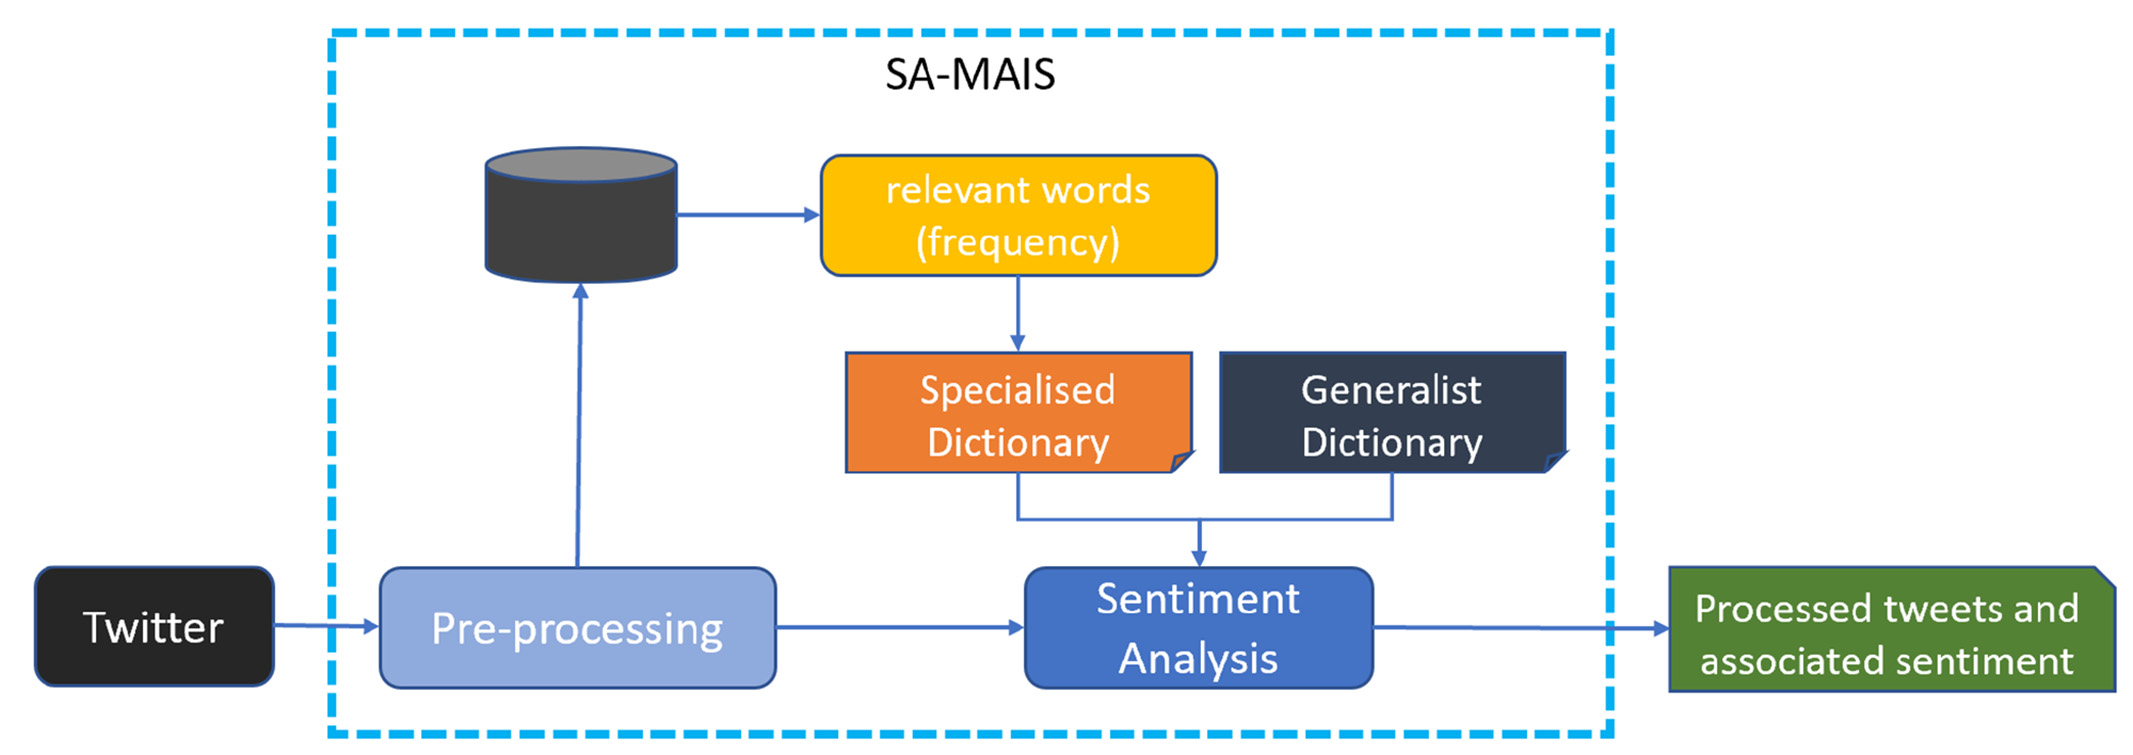
\includegraphics[width=0.85\linewidth]{gfx/m4l3_taborda_fig1_samais_architecture.png}
\par\smallskip{\small \textbf{Hình 1:} Kiến trúc hệ thống SA-MAIS.}
\end{figure}

Để kiểm định SA-MAIS như một bộ phân tích cảm xúc văn bản ngắn, chúng tôi khám phá và so sánh sáu bộ phân loại cảm xúc tổng quát nổi tiếng: TextBlob, Stanza, VADER, BERTweet, Twitter-roBERTa và FinBERT. Công cụ đầu tiên, TextBlob,\footnote{https://textblob.readthedocs.io.} là một thư viện Python được huấn luyện sẵn cho NLP, trả về hai giá trị cho phân tích cảm xúc: phân cực (polarity) của văn bản và tính chủ quan (subjectivity) của nó. Giá trị thứ hai là một thước đo mức độ thiếu tính khách quan và do đó mang tính trừu tượng, phụ thuộc vào nhận thức và quan điểm cá nhân, trong khi phân cực thể hiện cảm xúc tổng thể của tweet và được đánh giá trong khoảng $[-1.0, 1.0]$, với $-1.0$ là cảm xúc tiêu cực nhất và $1.0$ biểu thị cảm xúc hoàn toàn tích cực. Stanza [8] là một bộ công cụ được tạo ra vào năm 2020 tại Đại học Stanford để phân tích văn bản bằng nhiều ngôn ngữ (tiếng Anh, tiếng Đức và tiếng Trung). Bộ phân loại này được huấn luyện sử dụng 112 tập dữ liệu. Các giá trị phân cực khác với các giá trị trả về từ TextBlob vì Stanza trả về các giá trị 0, 1 và 2, đại diện tương ứng cho cảm xúc tiêu cực, trung lập và tích cực. Hutto và Gilbert [46] phát triển VADER, được coi là thư viện nhúng trong NLTK. Các tác giả mô tả VADER là ``một mô hình dựa trên quy tắc đơn giản cho phân tích cảm xúc tổng quát''. VADER đã được so sánh với các từ điển cảm xúc/quan điểm khác nhau: Linguistic Inquiry Word Count (LIWC), General Inquirer (GI), Affective Norms for English Words (ANEW), SentiWordNet (SWN), SenticNet (SCN) và Word-Sense Disambiguation (WSD) sử dụng WordNet. Các tác giả kết luận rằng VADER vượt trội hơn tất cả các từ điển khi phân loại văn bản mạng xã hội [9].

\begin{figure}[H]
\centering
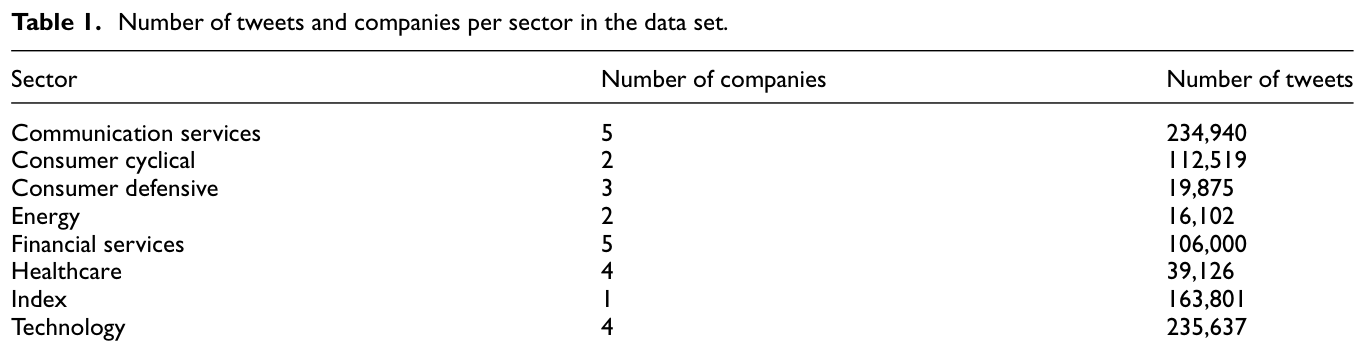
\includegraphics[width=0.9\linewidth]{gfx/m4l3_taborda_table1_tweets_per_sector.png}
\par\smallskip{\small \textbf{Bảng 1:} Số lượng tweet và số công ty theo từng ngành trong tập dữ liệu.}
\end{figure}

\begin{figure}[H]
\centering
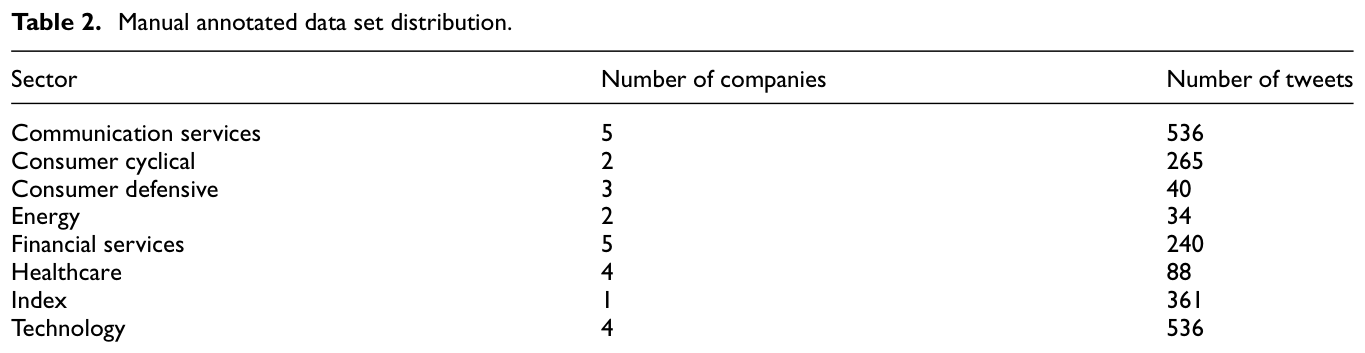
\includegraphics[width=0.9\linewidth]{gfx/m4l3_taborda_table2_annotated_data_distribution.png}
\par\smallskip{\small \textbf{Bảng 2:} Phân bố tập dữ liệu được gán nhãn thủ công.}
\end{figure}

BERTweet là một mô hình do Quoc Nguyen et al. [41] tạo ra, được huấn luyện với kho ngữ liệu SemEval 2017 (khoảng 40,000 tweet). Mô hình phân loại cảm xúc thành ba lớp khác nhau: POS, NEG và NEU, lần lượt đại diện cho cảm xúc tích cực, tiêu cực và trung lập. Twitter-roBERTa được huấn luyện trên khoảng 58 triệu tweet và được tinh chỉnh cho phân tích cảm xúc bằng bộ chuẩn TweetEval [44]. Mô hình đưa ra ba nhãn để phân loại cảm xúc, 0 đại diện cho cảm xúc tiêu cực, 1 đại diện cho cảm xúc trung lập và 2 đại diện cho cảm xúc tích cực. FinBERT được huấn luyện tinh chỉnh bằng Financial Phrasebank của Malo et al. [47]. Mô hình cho ra ba nhãn đầu ra: tích cực, tiêu cực và trung lập.

Cần lưu ý rằng, theo hiểu biết tốt nhất của chúng tôi, (1) không có tập dữ liệu tweet thị trường chứng khoán được gán nhãn thủ công cho ba lớp cảm xúc có thể có: tích cực, trung lập và tiêu cực. Hơn nữa, (2) không có bộ dữ liệu chuẩn (benchmark) với số lượng tweet đủ lớn liên quan đến S\&P500 và các công ty thành viên. Về vấn đề này, chúng tôi đã thu thập và lọc khoảng 928,000 tweet về thị trường chứng khoán, trong khoảng thời gian từ ngày 9 tháng 4 năm 2020 đến ngày 16 tháng 7 năm 2020, liên quan đến 25 công ty có khối lượng giao dịch cao nhất trong chỉ số S\&P 500 thông qua mã cổ phiếu (cash tag), \$SPX và \#stock. Khung thời gian này được sử dụng nhằm giảm khả năng xuất hiện các mô hình theo mùa/thời điểm (tức là xu hướng gia tăng của cảm xúc) có thể ảnh hưởng đến thực nghiệm và, do đó, ảnh hưởng đến kết quả. Bảng 1 cho thấy sự phân bố của các công ty và tweet theo từng ngành kinh tế.

Việc tạo ra một tập dữ liệu được gán nhãn cho một nhiệm vụ đặc thù lĩnh vực rất tốn thời gian và chịu ảnh hưởng lớn bởi tính chủ quan của người gán nhãn. Ví dụ, Li et al. [48] sử dụng hai tập dữ liệu được gán nhãn để đề xuất một phương pháp phân tích cảm xúc mới cho các đánh giá của người dùng bằng các mô hình học sâu. Cả hai tập dữ liệu đều có tập kiểm định, lần lượt với 2210 và 802 đánh giá. Mowlaei et al. [49] đề xuất một bộ phân tích cảm xúc theo khía cạnh (aspect-based sentiment analyser) mới. Để kiểm định mô hình này, các tác giả sử dụng một tập dữ liệu gồm 367 đánh giá tích cực và 267 đánh giá tiêu cực, tổng cộng 634 đánh giá. Chúng tôi không tìm thấy bất kỳ tập dữ liệu tweet nào được gán nhãn thủ công chuyên biệt cho lĩnh vực thị trường chứng khoán. Do đó, chúng tôi đã tự gán nhãn thủ công một mẫu ngẫu nhiên gồm 2100 tweet. Bảng 2 cho thấy sự phân bố công ty và tweet theo từng ngành kinh tế cho tập dữ liệu được gán nhãn thủ công này. Các tweet được phân loại thủ công bằng ba giá trị cảm xúc có sẵn: tích cực, trung lập và tiêu cực. Việc gán nhãn được thực hiện bởi hai người gán nhãn độc lập, là chuyên gia trong lĩnh vực thị trường chứng khoán, nhằm giảm tính chủ quan khi gán nhãn tập dữ liệu. Chỉ số kappa của Cohen [50] được sử dụng để định lượng mức độ đồng thuận giữa những người gán nhãn. Thước đo này nằm trong khoảng $[-1.0, 1.0]$, trong đó $1.0$ nghĩa là hoàn toàn đồng thuận giữa những người gán nhãn và $-1.0$ nghĩa là không có sự đồng thuận nào. Việc gán nhãn thủ công cho tập dữ liệu này đạt kappa 0.88, thể hiện mức độ đồng thuận gần như hoàn hảo giữa những người gán nhãn [50].

\section{5. Cải tiến từ điển cảm xúc}

Như đã chỉ ra trước đó, Loughran và McDonald đã tạo ra các danh sách cảm xúc dựa trên cách diễn giải khả dĩ nhất của một từ trong bối cảnh kinh doanh, tạo ra hai danh sách từ điển chứa 354 từ tích cực và 2329 từ tiêu cực [10]. Danh sách từ điển này từ đây được gọi là LMcD, hiện là một từ điển tài chính và kế toán tham chiếu [52]. Tuy nhiên, nó được xây dựng dựa trên các văn bản kế toán tài chính để tăng cường phân tích cảm xúc trong lĩnh vực đặc thù này.

Mục này mô tả các thay đổi được đưa vào từ điển LMcD nhằm cải thiện khả năng đại diện của nó cho việc phân tích thị trường chứng khoán (mục 5.1) và làm nổi bật các kết quả đạt được từ từ điển đã được tăng cường mới (mục 5.2).

\subsection*{5.1. LMcD20: cải tiến từ điển đặc thù lĩnh vực}

Một khảo sát sâu hơn về tập dữ liệu tweet thị trường chứng khoán thứ hai (tập dữ liệu chưa được gán nhãn) cho thấy một số từ đặc thù và phổ biến liên quan đến thị trường chứng khoán (như ``breakthrough'' và ``barred'') không được các công cụ phân tích cảm xúc tổng quát phân loại một cách phù hợp, cho thấy sự cần thiết phải sử dụng các từ điển đặc thù lĩnh vực. Tuy nhiên, một khảo sát chi tiết hơn về LMcD cũng cho thấy một số từ hiện đang được sử dụng trong các tweet tài chính vẫn chưa có mặt trong LMcD. Chúng tôi cũng nhận thấy rằng các từ dùng để bày tỏ quan điểm trên Twitter chịu ảnh hưởng của cách diễn giải chủ quan và thay đổi theo thời gian. Do đó, một từ điển đặc thù lĩnh vực cho Twitter không thể là tĩnh mà cần được điều chỉnh theo thời gian dựa trên nội dung từ vựng thực tế và cập nhật.

Để giải quyết vấn đề này, chúng tôi đã sử dụng dữ liệu tweet thị trường chứng khoán chứa dữ liệu mới hơn như một phương tiện để cải thiện từ điển của mình. Một mẫu các từ tích cực và tiêu cực chưa có trong LMcD được chọn từ 500 từ phổ biến nhất được trích xuất từ tập dữ liệu quy mô lớn. Trong số đó, 23 từ thể hiện cảm xúc tích cực (như ``buy'' hoặc ``bull'') và 13 từ thể hiện cảm xúc tiêu cực (như ``short'' hoặc ``bear''). Các tác giả đã lựa chọn thủ công các từ thể hiện cảm xúc, dẫn đến 36 từ mới liên quan đến tài chính (Bảng 3) được thêm vào từ điển LMcD, từ đó tạo ra LMcD20.

\begin{figure}[H]
\centering
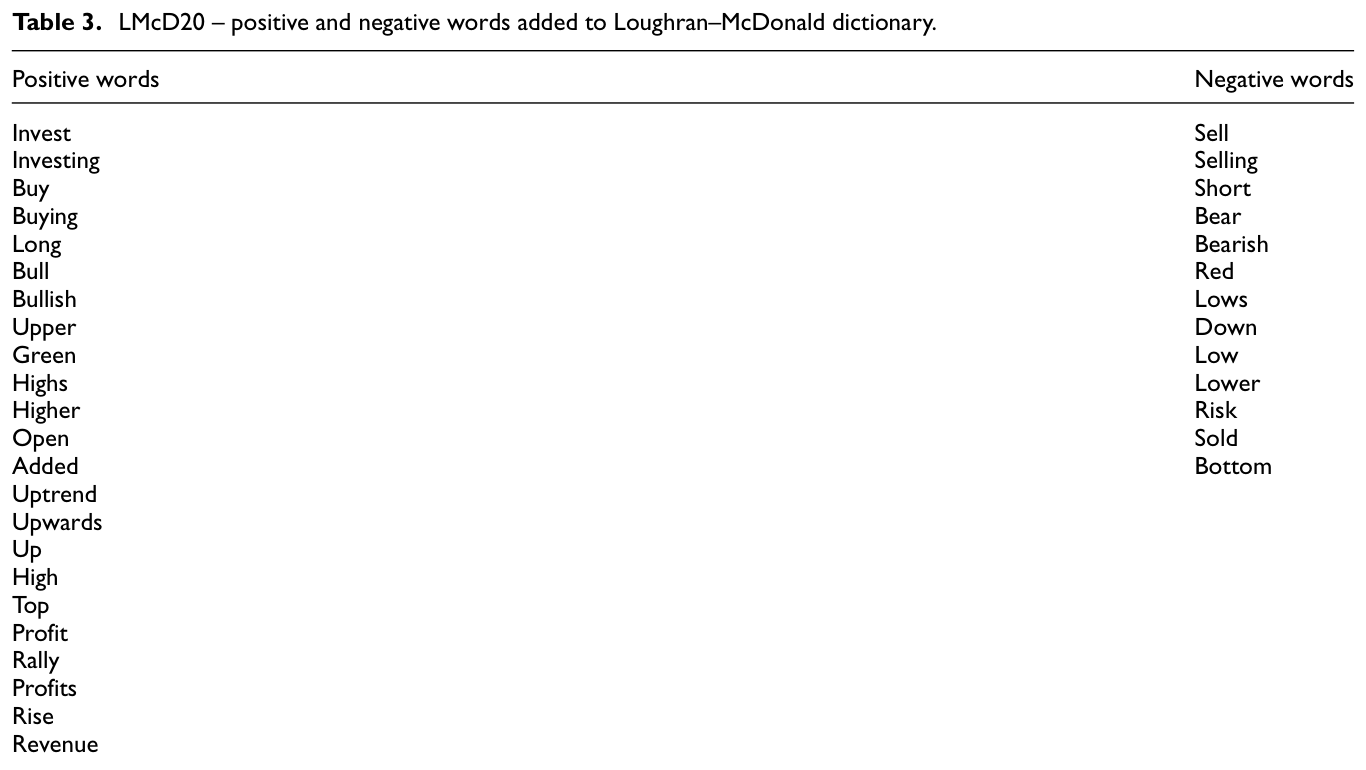
\includegraphics[width=0.85\linewidth]{gfx/m4l3_taborda_table3_lmcd20_words.png}
\par\smallskip{\small \textbf{Bảng 3:} LMcD20, các từ tích cực và tiêu cực được thêm vào từ điển Loughran\textendash McDonald.}
\end{figure}

Để giữ cho SA-MAIS cập nhật nhất có thể dựa trên tần suất từ, chúng tôi đã tạo ra một tập dữ liệu khác với gần 1 triệu tweet, cung cấp dữ liệu chất lượng quy mô lớn cho việc phân tích. Cả hai tập dữ liệu đều đã được công bố công khai [51].

\subsection*{5.2. So sánh các từ điển khác nhau}

Để đánh giá mô hình, tức là kiểm định kết quả phân loại tích cực, tiêu cực hoặc trung lập của các từ, và do lớp tiêu cực mất cân bằng nhẹ so với các lớp còn lại, thước đo được chọn để so sánh các thực nghiệm là độ nhạy trung bình có trọng số (weighted average recall, WAR). Hàm này gán trọng số cho recall của từng lớp theo số lượng mẫu của lớp đó. WAR được định nghĩa theo phương trình (1), trong đó $TP_p$, $TP_n$ và $TP_t$ lần lượt là số lượng dự đoán đúng (true positive) liên quan đến lớp tích cực ($p$), lớp tiêu cực ($n$) và lớp trung lập ($t$), còn $N$ đại diện cho tổng số tweet:

\[
\text{WAR} = \frac{TP_p + TP_n + TP_t}{N} \qquad (1)
\]

Trong thực nghiệm ban đầu, chúng tôi đã thực hiện so sánh giữa các từ điển đặc thù lĩnh vực. Trong các từ điển đặc thù lĩnh vực, Hu et al. [24] (Sentilex) là một trong những từ điển nổi tiếng nhất và được tạo ra để phân tích các đánh giá của khách hàng. Oliveira et al. [11] (từ điển cảm xúc thị trường chứng khoán, SMSL) và Loughran và McDonald [10] (LMcD) là ví dụ về các từ điển tài chính được tạo ra để sử dụng trong các bối cảnh kinh tế cụ thể. Mohammad và Turney [53] (NRC) là một trong những từ điển đặc thù lĩnh vực nổi tiếng nhất kết hợp phân cực cảm xúc và cảm xúc trong cùng một từ điển cho một kịch bản huy động cộng đồng (crowd-sourcing). Loughran và McDonald tạo ra từ điển LMcD vào năm 2011 để đánh giá các báo cáo tài chính của các công ty. LMcD chứa hai tập con từ: tập từ tiêu cực, bao gồm 2329 từ, và tập từ tích cực, chứa 354 từ [10]. Nhiều từ liên quan đến thị trường tài chính có thể được tìm thấy trong từ điển, nhưng khác với tweet, các báo cáo tài chính được cấu trúc rất tốt và được viết cẩn thận.

Từ điển SMSL được tạo ra vào năm 2016 với mục tiêu chính là đánh giá cảm xúc StockTwits [11]. Từ điển này chứa 20,551 uni-gram và bi-gram và được tạo tự động dựa trên một mẫu StockTwits sử dụng phương pháp thống kê. Tuy vậy, việc kiểm định SMSL được thực hiện bằng cách sử dụng một lựa chọn gồm 5000 StockTwits được các tác giả của các bài đăng phân loại nhưng loại trừ cảm xúc trung lập. Mỗi $n$-gram ($n = 1, 2$) có một trọng số khác nhau tùy theo ngữ cảnh của câu tại thời điểm đó, mang tính tích cực hoặc tiêu cực. SMSL được tạo tự động dựa trên một tập dữ liệu từ StockTwits, nhưng không giống tweet, trọng tâm chính của StockTwits là độc giả liên quan đến thị trường tài chính.

Hình 2 cho thấy kết quả phân tích cảm xúc khi sử dụng từng từ điển đặc thù lĩnh vực. Có thể thấy rằng SMSL cho kết quả WAR thấp nhất (40.0\%). Một trong những lý do khiến kết quả của SMSL thấp có thể là vì nó được tạo tự động sử dụng StockTwits. Nền tảng này khác với Twitter và ngôn ngữ được sử dụng có tính chuyên biệt và định hướng nhiều hơn, chủ yếu dành cho độc giả thị trường tài chính. Một lý do thứ hai là SMSL sử dụng uni-gram và bi-gram được tạo tự động với tập dữ liệu StockTwits. Đáng chú ý là hai từ điển đặc thù lĩnh vực tốt nhất khi được kết hợp lại, cụ thể là Sentilex và LMcD. Dựa trên Hình 2, Sentilex kết hợp với LMcD vượt trội hơn LMcD đơn lẻ 1.4 điểm phần trăm (p.p.). So sánh LMcD với các từ điển đặc thù lĩnh vực còn lại (NRC và Sentilex), LMcD vượt trội hơn cả hai lần lượt là 8 p.p. và 0.5 p.p.

\begin{figure}[H]
\centering
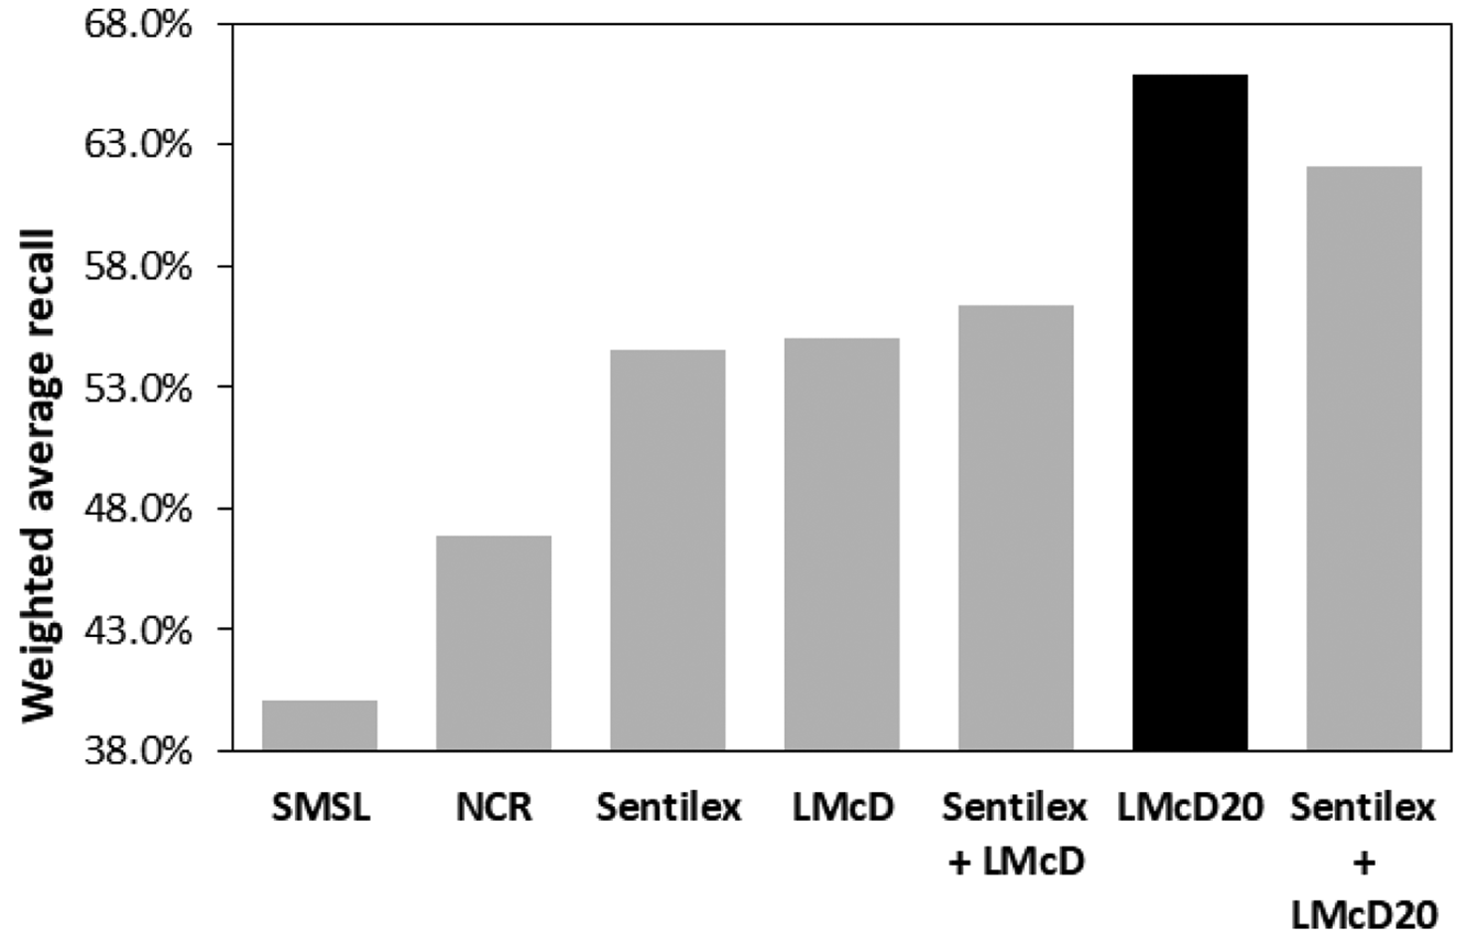
\includegraphics[width=0.85\linewidth]{gfx/m4l3_taborda_fig2_comparing_lexicons_war.png}
\par\smallskip{\small \textbf{Hình 2:} So sánh các từ điển cảm xúc, độ nhạy trung bình có trọng số (WAR).}
\end{figure}

Trong nỗ lực cải thiện WAR tổng thể, LMcD20 đã được tạo ra như đã mô tả trước đó ở mục 5.1. Đáng chú ý, việc sử dụng độc lập LMcD20 đạt hiệu suất tốt nhất (65.9\%) so với các từ điển còn lại. Cụ thể, LMcD20 cho thấy mức cải thiện 11 p.p. so với LMcD. Có sự sụt giảm về WAR khi kết hợp Sentilex và LMcD20. Sụt giảm này chủ yếu do LMcD20 đặc thù cho các tweet thị trường chứng khoán, còn Sentilex đặc thù cho các đánh giá của khách hàng.

Mặc dù kết quả của LMcD20 có thể được coi là thỏa đáng, một phân tích kỹ lưỡng các kết quả cho thấy rằng một từ điển đơn từ (uni-gram) như LMcD20 vẫn còn hạn chế trong việc phân loại cảm xúc tweet. Do đó, chúng tôi nhận thấy cần phải kết hợp một GSA với từ điển đặc thù lĩnh vực này, điều đã được thực hiện thông qua việc triển khai SA-MAIS như mô tả ở mục 6.

\section{6. SA-MAIS: phương pháp lai để phân tích tweet thị trường chứng khoán}

Mục này trình bày chi tiết việc triển khai SA-MAIS. Mục 6.1 mô tả cách kết hợp GSA và các từ điển đặc thù lĩnh vực, còn mục 6.2 làm nổi bật các kết quả đạt được với việc triển khai này.

\subsection*{6.1. Phân loại tweet}

Để đạt được hiệu suất tốt nhất, SA-MAIS kết hợp một bộ phân loại cảm xúc tổng quát, chẳng hạn như thư viện TextBlob, bộ công cụ Stanza, VADER, BERTweet, Twitter-roBERTa, FinBERT, và một từ điển đặc thù lĩnh vực (như SMSL, NRC, Sentilex, LMcD hoặc từ điển LMcD20 đã được tăng cường). Kỹ thuật này dựa vào việc sử dụng đồng thời cả hai công cụ cho phân tích văn bản và tích hợp kết quả phân loại bằng một tổ hợp lồi (convex combination).

\subsubsection*{6.1.1. Thành phần GSA}

Như đã đề cập trước đó, TextBlob trả về phân cực thể hiện cảm xúc tổng thể của tweet: một giá trị trong khoảng $[-1.0, 1.0]$, với $-1.0$ thể hiện cảm xúc hoàn toàn tiêu cực và $1.0$ là cảm xúc hoàn toàn tích cực. VADER cũng báo cáo phân cực trong cùng khoảng giá trị, nhưng kết quả của Stanza là 0, 1 hoặc 2, lần lượt đại diện cho cảm xúc tiêu cực, trung lập hoặc tích cực. Ba mô hình học sâu dựa trên BERT được sử dụng trong bài báo này, cụ thể là BERTweet, Twitter-roBERTa và FinBERT, đưa ra ba lớp đại diện cho cảm xúc được phân tích trong văn bản. Mặc dù các nhãn được biểu diễn khác nhau như đã đề cập trước đó, tất cả các mô hình đều có xu hướng biểu diễn cảm xúc tích cực, tiêu cực và trung lập.

Điều này có nghĩa là, bất kể công cụ nào được sử dụng, giá trị phân cực cảm xúc do thành phần GSA của SA-MAIS đưa ra là một giá trị $P_0 \in [-1.0, 1.0]$. Do đó, trong khi giá trị trả về ($pol$) từ các bộ phân tích cảm xúc tổng quát TextBlob và VADER được lấy theo giá trị thực của chúng, trong trường hợp sử dụng Stanza, đầu ra của nó được chuyển đổi thành $-1$, $0$ hoặc $1$, lần lượt biểu thị cảm xúc tiêu cực, trung lập hoặc tích cực. Tương tự phép chuyển đổi của Stanza, đầu ra của BERTweet, Twitter-roBERTa và FinBERT được chuyển đổi thành $-1$, $0$ hoặc $1$, lần lượt biểu thị cảm xúc tiêu cực, trung lập hoặc tích cực. Phương trình (2) định nghĩa giá trị phân cực GSA cho SA-MAIS, trong đó $pol$ đại diện cho cảm xúc do một GSA cụ thể đưa ra và các biến thể BERT đại diện cho các mô hình được sử dụng trong nghiên cứu này (BERTweet, Twitter-roBERTa và FinBERT):

\[
P_0 =
\begin{cases}
pol - 1, & \text{nếu } pol \text{ là đầu ra của Stanza} \\
-1, & \text{nếu } pol \text{ là tiêu cực từ một mô hình dựa trên BERT} \\
0, & \text{nếu } pol \text{ là trung lập từ một mô hình dựa trên BERT} \\
1, & \text{nếu } pol \text{ là tích cực từ một mô hình dựa trên BERT} \\
pol, & \text{trường hợp còn lại}
\end{cases}
\qquad (2)
\]

\subsubsection*{6.1.2. Thành phần từ điển đặc thù lĩnh vực}

Thành phần đặc thù lĩnh vực của SA-MAIS phân loại từng tweet bằng cách so sánh nội dung của nó với một từ điển đặc thù lĩnh vực ở cấp độ từ. Gọi $W_{\text{pos}}$ là số lượng từ trùng khớp trong tập từ tích cực, và $W_{\text{neg}}$ là số lượng từ trùng khớp trong tập từ tiêu cực. Đầu ra của thành phần này được tính theo phương trình (3):

\[
P_1 =
\begin{cases}
\dfrac{(W_{\text{pos}} - W_{\text{neg}})}{(W_{\text{pos}} + W_{\text{neg}})}, & \text{nếu } (W_{\text{pos}} + W_{\text{neg}}) > 0 \\[2mm]
0, & \text{trường hợp còn lại}
\end{cases}
\qquad (3)
\]

Trong trường hợp không có từ nào của tweet trùng khớp với từ điển đặc thù lĩnh vực, đầu ra của thành phần từ điển đặc thù lĩnh vực bằng 0.

\begin{figure}[H]
\centering
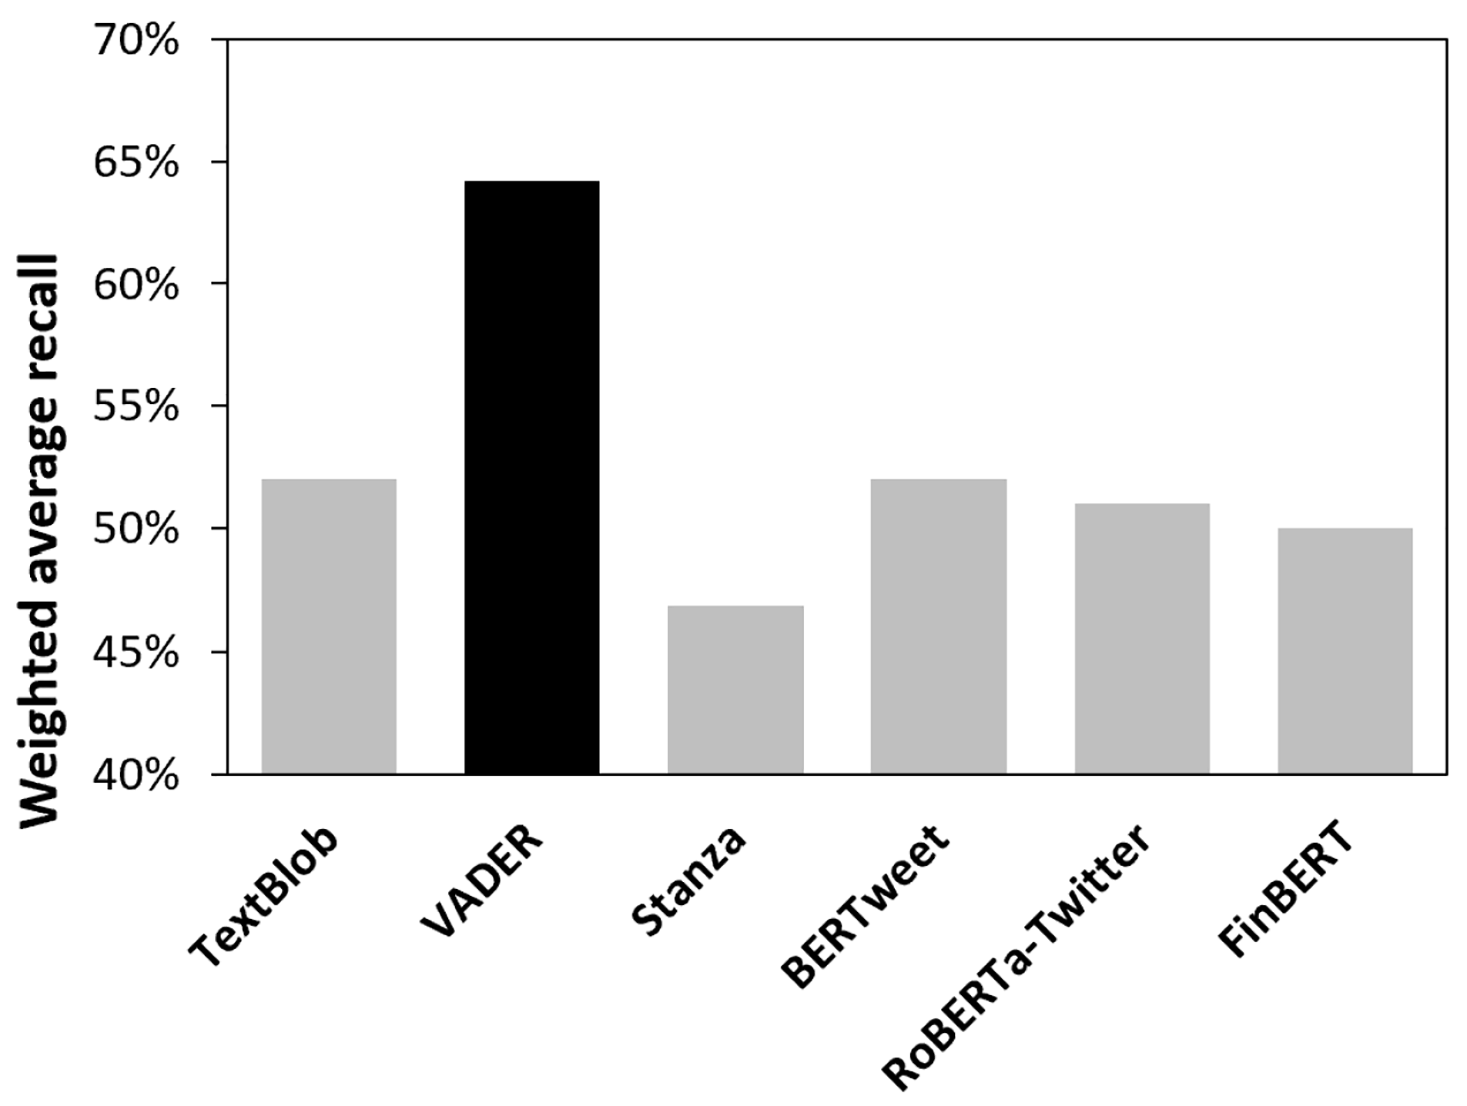
\includegraphics[width=0.75\linewidth]{gfx/m4l3_taborda_fig3_comparing_generalist_sa.png}
\par\smallskip{\small \textbf{Hình 3:} So sánh hiệu suất của các công cụ phân tích cảm xúc tổng quát trên tập dữ liệu của chúng tôi.}
\end{figure}

\subsubsection*{6.1.3. Bộ tích hợp giá trị cảm xúc của SA-MAIS}

Đầu ra của SA-MAIS là một tổ hợp lồi tuyến tính của hai thành phần trước đó, được cho bởi phương trình (4), trong đó $P_0$ là phân cực của GSA, $P_1$ là đầu ra của từ điển đặc thù lĩnh vực, và $\lambda$ là một tham số xác định tầm quan trọng của từ điển đặc thù lĩnh vực trong kết quả cuối cùng. Vì $\lambda \in [0.0, 1.0]$, khoảng giá trị của phân cực không bị thay đổi:

\[
P = (1 - \lambda) \times P_0 + \lambda \times P_1 \qquad (4)
\]

Cuối cùng, phương trình (5) định nghĩa đầu ra dạng phân loại (categorical) của SA-MAIS. Mỗi tweet được phân loại là tiêu cực, trung lập hoặc tích cực, theo giá trị $P$ được cho bởi phương trình (4). Tham số $\beta$ phụ thuộc vào GSA được sử dụng: $\beta = 0.0$ khi sử dụng TextBlob, Stanza, BERTweet, Twitter-roBERTa hoặc FinBERT, và $\beta = 0.05$ khi sử dụng VADER, vì các tác giả của VADER coi một giá trị trong khoảng từ $-0.05$ đến $0.05$ là trung lập:

\[
C =
\begin{cases}
\text{tiêu cực}, & -1.0 \leq P < \beta \\
\text{trung lập}, & -\beta \leq P \leq \beta \\
\text{tích cực}, & \beta < P \leq 1.0
\end{cases}
\qquad (5)
\]

\subsection*{6.2. Kết quả}

Thực nghiệm đầu tiên nhằm thiết lập đường cơ sở (baseline), gồm đánh giá hiệu suất của TextBlob, Stanza, VADER, BERTweet, Twitter-roBERTa và FinBERT khi được sử dụng độc lập trên tập dữ liệu được gán nhãn. Điều này có nghĩa là thực nghiệm được thực hiện bằng cách đặt tham số $\lambda = 0$ trong phương trình (4), và do đó, các từ điển đặc thù lĩnh vực không được sử dụng.

Như thể hiện trong Hình 3, VADER vượt trội rõ rệt so với các công cụ còn lại, đạt WAR xấp xỉ 64.0\% so với 52.0\% của BERTweet, mô hình đạt WAR cao nhất trong số các mô hình còn lại được so sánh. Như vậy, trong số các công cụ được so sánh, VADER nổi bật là bộ phân loại phù hợp nhất cho phân tích cảm xúc tweet thị trường chứng khoán.

So sánh các ma trận nhầm lẫn (confusion matrices) phân loại của TextBlob và VADER (Bảng 4 và Bảng 5), có thể thấy rằng TextBlob có tỷ lệ sai sót cao hơn ở lớp cảm xúc tích cực so với khi dự đoán lớp trung lập hoặc lớp tiêu cực. Ngược lại, mặc dù VADER cho thấy một ma trận nhầm lẫn đồng đều hơn, có thể thấy rằng nó chủ yếu sai sót khi phân loại các tweet có cảm xúc tiêu cực. Về ma trận nhầm lẫn của BERTweet (Bảng 6), mô hình này chủ yếu sai sót ở các lớp cảm xúc tích cực và tiêu cực, phân loại nhiều tweet trong số đó là trung lập. Do đó, dường như mô hình này hoặc đang thiếu ngữ cảnh hoặc thiếu các từ có phân cực đặc thù lĩnh vực để đạt được phân loại phù hợp cho các tweet tài chính liên quan đến thị trường chứng khoán.

\begin{figure}[H]
\centering
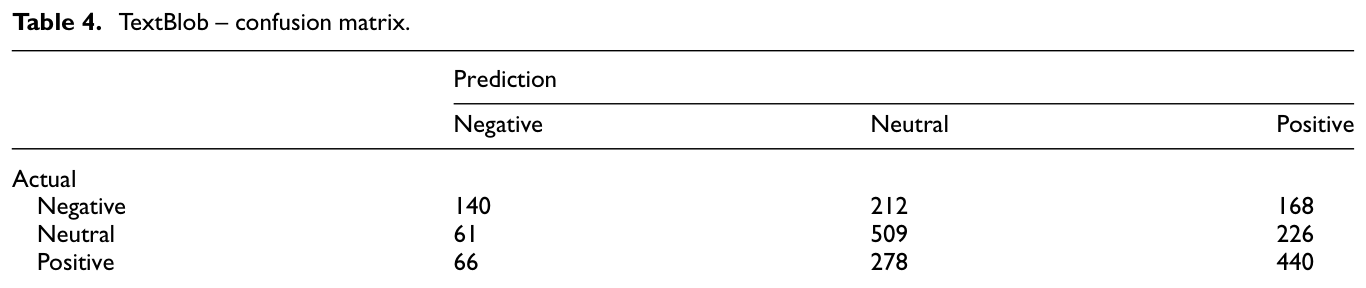
\includegraphics[width=0.85\linewidth]{gfx/m4l3_taborda_table4_textblob_confusion.png}
\par\smallskip{\small \textbf{Bảng 4:} Ma trận nhầm lẫn của TextBlob.}
\end{figure}

\begin{figure}[H]
\centering
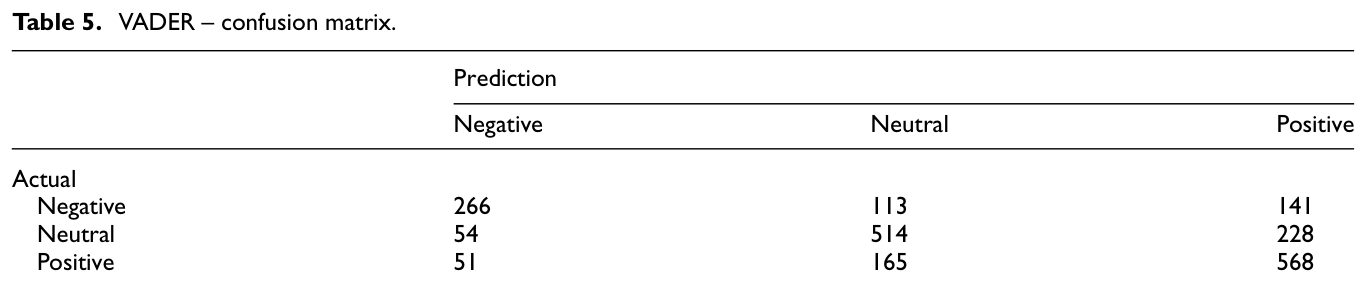
\includegraphics[width=0.85\linewidth]{gfx/m4l3_taborda_table5_vader_confusion.png}
\par\smallskip{\small \textbf{Bảng 5:} Ma trận nhầm lẫn của VADER.}
\end{figure}

\begin{figure}[H]
\centering
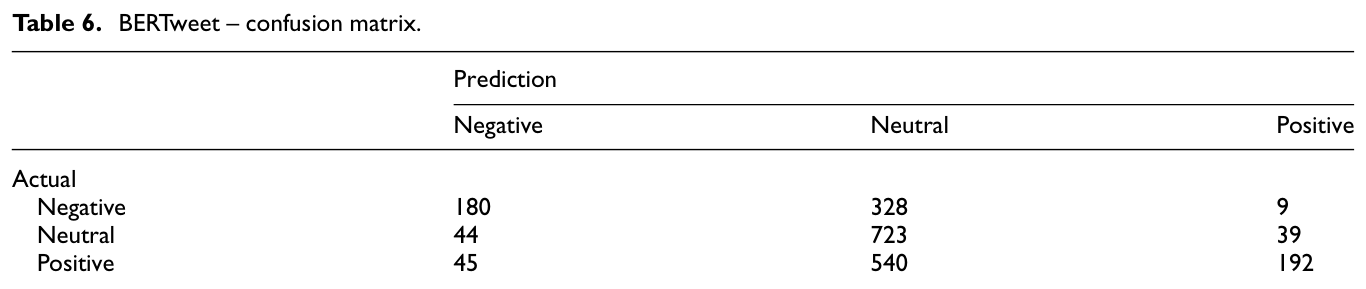
\includegraphics[width=0.85\linewidth]{gfx/m4l3_taborda_table6_bertweet_confusion.png}
\par\smallskip{\small \textbf{Bảng 6:} Ma trận nhầm lẫn của BERTweet.}
\end{figure}

Với các kết quả trên, cách tiếp cận tích hợp của SA-MAIS được đánh giá bằng cách sử dụng VADER làm thành phần tổng quát kết hợp với LMcD20, từ điển đạt kết quả tốt nhất trong các thực nghiệm ở mục 5.2.

Như có thể quan sát trong Hình 4, WAR của việc phân loại cảm xúc đã tăng từ 65.9\% với LMcD20 và 64.0\% với VADER lên đến 71.8\% với VADER + LMcD20. Như vậy, có một mức tăng tổng thể 6 p.p. so với LMcD20 sử dụng độc lập và 8 p.p. so với VADER sử dụng độc lập. Lưu ý rằng kết quả tốt nhất đạt được tại $\lambda = 0.5$, nghĩa là cả hai thành phần có tỷ trọng đóng góp bằng nhau vào việc phân loại cảm xúc cuối cùng của tweet.

\begin{figure}[H]
\centering
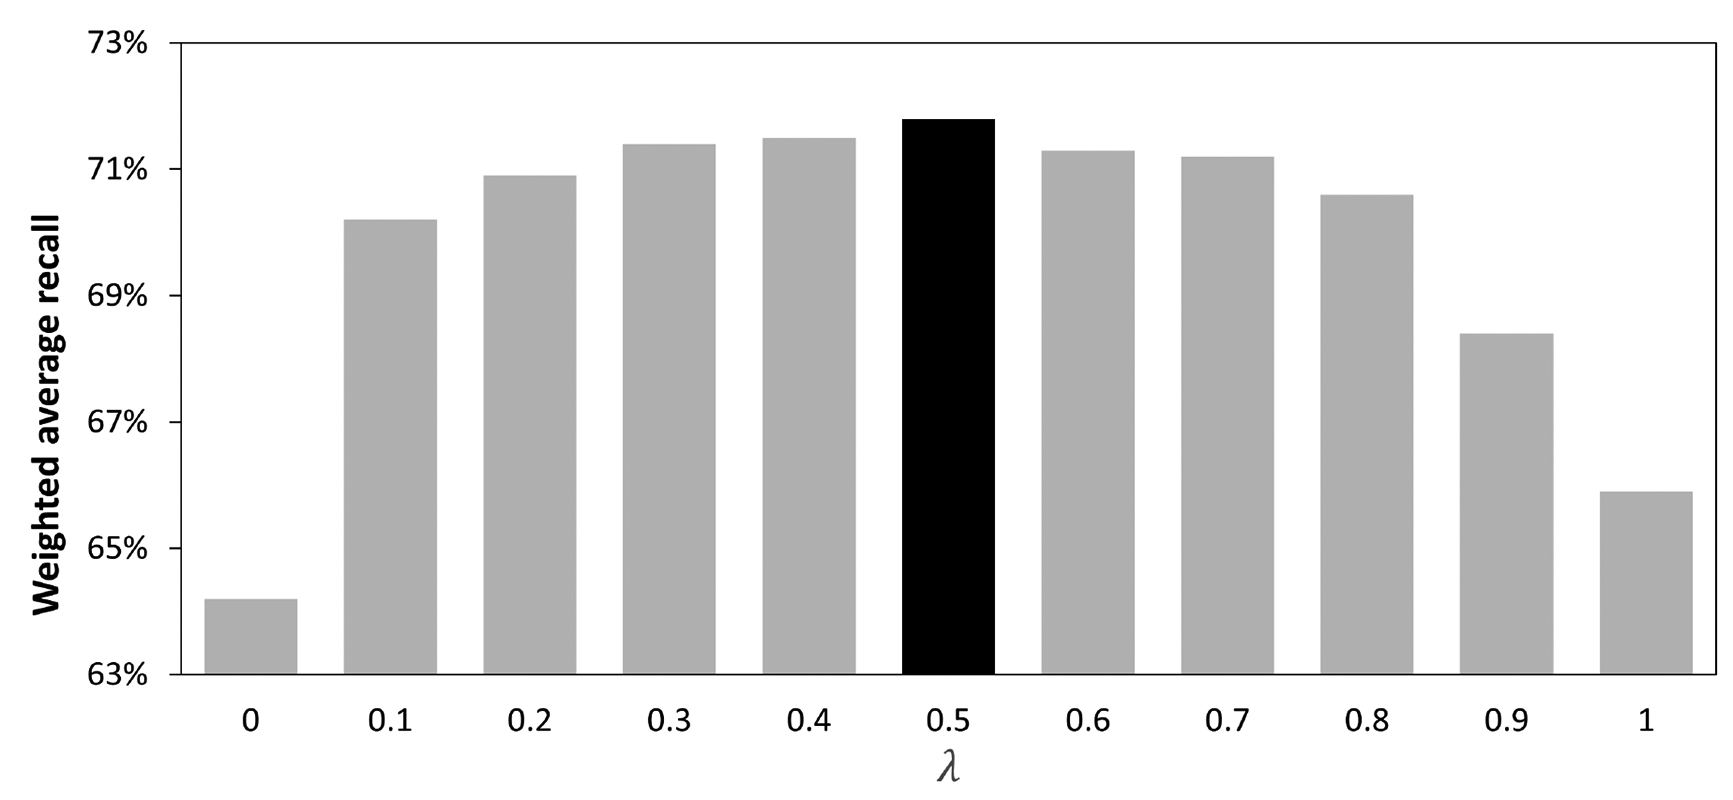
\includegraphics[width=0.75\linewidth]{gfx/m4l3_taborda_fig4_lmcd20_vader_lambda.png}
\par\smallskip{\small \textbf{Hình 4:} So sánh hiệu suất của LMcD20 và VADER theo các giá trị khác nhau của $\lambda$.}
\end{figure}

Các giá trị thước đo tổng thể cho SA-MAIS khi sử dụng VADER cộng với LMcD20 với $\lambda = 0.5$ được trình bày trong Bảng 7, cho biết chi tiết hành vi của SA-MAIS đối với từng lớp cảm xúc bằng cách hiển thị các thước đo đánh giá phổ biến nhất (precision, recall và F1-score). Về recall, số liệu thống kê cho thấy phân loại hiệu quả nhất là dành cho lớp tích cực, với giá trị 87.1\%. Lớp cảm xúc tiêu cực cho giá trị recall 71.4\%, còn lớp trung lập có giá trị recall thấp nhất là 57.8\%. Giá trị precision thấp nhất, 64.6\%, đạt được ở lớp tích cực, trong khi lớp trung lập là lớp có precision cao nhất, đạt 82.9\%. Theo các kết quả trên, các lớp có F1-score tốt nhất là lớp tích cực và lớp tiêu cực, lần lượt đạt 74.2\% và 73.6\%. Nhìn chung, F1-score trung bình có trọng số của SA-MAIS là 71.7\%.

\begin{figure}[H]
\centering
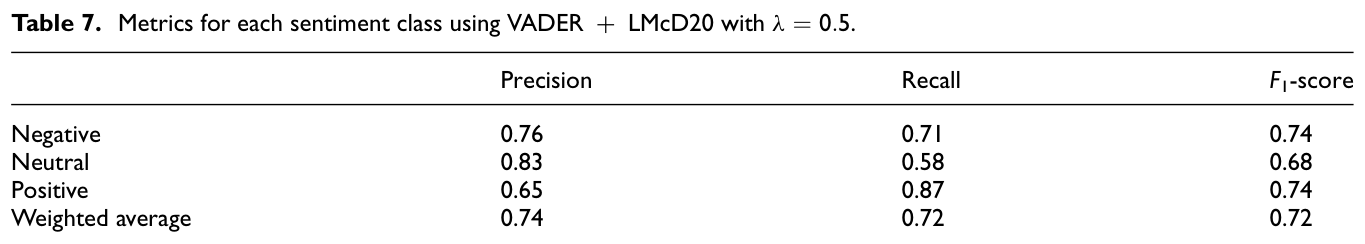
\includegraphics[width=0.6\linewidth]{gfx/m4l3_taborda_table7_metrics_vader_lmcd20.png}
\par\smallskip{\small \textbf{Bảng 7:} Các thước đo cho từng lớp cảm xúc khi sử dụng VADER + LMcD20 với $\lambda = 0.5$.}
\end{figure}

Để minh họa rõ hơn thế nào là một tweet tích cực, trung lập và tiêu cực, Bảng 8 trình bày một ví dụ về dự đoán đúng của SA-MAIS cho từng lớp cảm xúc này.

\begin{figure}[H]
\centering
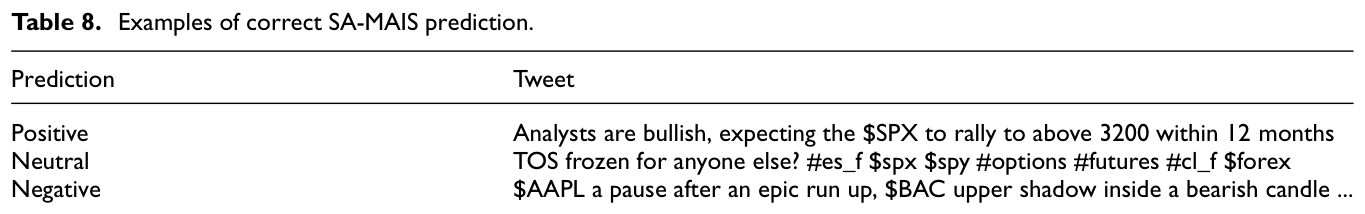
\includegraphics[width=0.9\linewidth]{gfx/m4l3_taborda_table8_correct_prediction_examples.png}
\par\smallskip{\small \textbf{Bảng 8:} Ví dụ về các dự đoán đúng của SA-MAIS.}
\end{figure}

\section{7. Đóng góp và hàm ý thực tiễn}

Nghiên cứu này đề xuất một phương pháp tham số lai (hybrid parametric approach) để phân tích phân cực cảm xúc của các thông điệp văn bản ngắn, kết hợp một bộ phân tích cảm xúc tổng quát với một từ điển đặc thù lĩnh vực đã được cập nhật, gọi là SA-MAIS.

Nghiên cứu cung cấp những hiểu biết mới về phân tích cảm xúc đặc thù lĩnh vực đối với văn bản ngắn trên mạng xã hội. Nó mô tả một cách tiếp cận phương pháp luận mới và cho thấy rằng (a) một cách đơn giản nhưng hiệu quả để tích hợp vốn từ vựng cập nhật theo thời gian từ văn bản ngắn đặc thù lĩnh vực mang lại giá trị gia tăng cho các nhiệm vụ phân loại, và (b) việc sử dụng từ điển đã được tăng cường này cải thiện các công cụ phân tích cảm xúc tổng quát hiện có, cung cấp một công cụ chính xác hơn để phân tích cảm xúc văn bản trong một ngôn ngữ chuyên biệt kỹ thuật cụ thể. Cụ thể, chúng tôi mô tả một bằng chứng khái niệm của phương pháp luận này bằng cách áp dụng nó vào việc phân tích và dự đoán tweet thị trường chứng khoán. Mặc dù trọng tâm của nghiên cứu này là thị trường chứng khoán, cách tiếp cận tổng quát có thể được áp dụng cho các lĩnh vực khác nhau, dù là tài chính hay không, bằng cách thay thế từ điển đặc thù và sử dụng các tweet từ lĩnh vực được chọn để tăng cường từ điển mới.

Thứ hai, nghiên cứu đóng góp cho lĩnh vực học máy và khai phá văn bản (text mining) bằng cách cung cấp một kho ngữ liệu thị trường chứng khoán mới được gán nhãn để làm chuẩn so sánh cho các phương pháp và kỹ thuật mới. Thứ ba, bằng cách so sánh hiệu suất của một số công cụ tổng quát hiện có, nghiên cứu cho thấy rằng các công cụ này, khi sử dụng độc lập, phần lớn không đủ để phân loại chính xác và chi tiết cảm xúc của các tweet liên quan đến thị trường chứng khoán.

\section{8. Kết luận}

Một phương pháp phân tích cảm xúc mới, SA-MAIS, sử dụng một khung dựa trên việc tích hợp có kiểm soát một GSA và một từ điển đặc thù lĩnh vực đã được trình bày. Hệ thống này kết hợp GSA nổi tiếng VADER với một từ điển đặc thù lĩnh vực, LMcD20, được cập nhật với các xu hướng từ vựng gần đây hơn. Một phiên bản được tăng cường của từ điển tài chính LMcD, có tên LMcD20, tích hợp các từ mới hơn và cập nhật liên quan đến tài chính, được tự động rút trích từ các tweet thị trường chứng khoán, cũng đã được trình bày.

Phương pháp kết hợp lai của SA-MAIS giữa phân tích tổng quát và đặc thù lĩnh vực đã được kiểm định toàn diện bằng cách sử dụng sáu GSA phổ biến: TextBlob, Stanza [8], VADER [9] và các mô hình tiên tiến được huấn luyện chuyên biệt BERTweet [41], Twitter-roBERTa và FinBERT [42], cùng với bốn từ điển tài chính chuyên biệt hiện có: từ điển cảm xúc tài chính LMcD [10], SMSL [11], Sentilex [24] và NRC [53]. Là một bằng chứng khái niệm, sau khi thực hiện một số thực nghiệm, có thể kết luận rằng từ điển mới được tăng cường LMcD20 cho thấy mức tăng khoảng sáu điểm phần trăm về kết quả WAR đối với kho ngữ liệu Twitter thị trường chứng khoán. Hơn nữa, việc triển khai SA-MAIS bằng cách tích hợp VADER với LMcD20 đã cải thiện các kết quả trước đó trên tất cả các lớp phân loại có thể, tích cực, tiêu cực và trung lập. Những kết quả này cho thấy SA-MAIS có thể được sử dụng như một công cụ trong các hệ thống phức tạp hơn để dự đoán diễn biến thị trường, vì nó vượt trội hơn các mô hình NLP tiên tiến nhất sử dụng học sâu.

Cuối cùng, tất cả các thực nghiệm được tiến hành sử dụng một kho ngữ liệu mới được gán nhãn, công bố công khai tại \url{https://github.com/taborda11/SAMAIS}. Về các hướng nghiên cứu tiếp theo, nghiên cứu này tất yếu vẫn còn một số hạn chế. Lý tưởng nhất, tập dữ liệu gồm 2100 tài liệu được gán nhãn nên được mở rộng, vì việc gán nhãn thủ công thêm các tweet không chỉ giúp làm giàu kho ngữ liệu đã gán nhãn mà còn là một tài sản quan trọng cho việc tăng cường LMcD20 trong tương lai, từ đó cải thiện kết quả phân loại cảm xúc của SA-MAIS. Thứ hai, các từ điển phức tạp hoặc có mục đích hơn, có thể đại diện cho các mối quan hệ giữa các từ và thêm thông tin ngôn ngữ, có thể đóng vai trò then chốt trong việc cải thiện các kết quả được trình bày ở đây. Thứ ba, các thử nghiệm trực tuyến (online tests) với SA-MAIS có thể cải thiện hiệu suất của công cụ này và mở rộng phạm vi ứng dụng.

\section*{Tuyên bố xung đột lợi ích}

Các tác giả tuyên bố không có xung đột lợi ích tiềm ẩn nào liên quan đến việc nghiên cứu, viết bài và/hoặc xuất bản bài báo này.

\section*{Tài trợ}

Các tác giả công bố đã nhận được hỗ trợ tài chính sau đây cho việc nghiên cứu, viết bài và/hoặc xuất bản bài báo này: Nghiên cứu này được tài trợ một phần bởi nguồn ngân sách quốc gia thông qua Fundação para a Ciência e a Tecnologia (FCT) với các mã số tham chiếu UIDB/50021/2020 và UIDB/00315/2020.

\section*{Ghi chú}

\begin{enumerate}
  \item https://github.com/taborda11/SAMAIS.
  \item https://ieee-dataport.org/open-access/stock-market-tweets-data.
  \item https://stocktwits.com.
  \item https://textblob.readthedocs.io.
\end{enumerate}

\section*{ORCID iD}

Bruno Taborda \url{https://orcid.org/0000-0002-3564-8662}

% [Đã lược bỏ danh mục Tài liệu tham khảo gốc (tiếng Anh, trích dẫn của tác giả bài gốc) để giảm dung lượng chương; không ảnh hưởng nội dung học thuật chính.]
